\documentclass[10pt,a4paper]{article}

% Essential packages
\usepackage[utf8]{inputenc}
\usepackage[T1]{fontenc}
\usepackage{amsmath,amsfonts,amssymb}
\usepackage{graphicx}
\usepackage{subcaption}
\usepackage{booktabs}
\usepackage{multirow}
\usepackage{multicol}
\usepackage{array}
\usepackage{tabularx}
\usepackage{longtable}
\usepackage{times} % More compact font

% Page layout
\usepackage[margin=0.8in]{geometry}
\usepackage{setspace}
\singlespacing

% Bibliography and citations
\usepackage[style=authoryear,backend=biber,natbib=true]{biblatex}
\addbibresource{references.bib}

% Colors and links
\usepackage{xcolor}
\usepackage[colorlinks=true,citecolor=blue,linkcolor=black,urlcolor=blue]{hyperref}

% Additional packages for better formatting
\usepackage{caption}
\usepackage{float}
\usepackage{enumitem}
\usepackage{textcomp}
\usepackage{microtype}

% Custom commands
\newcommand{\todo}[1]{\textcolor{red}{\textbf{TODO: #1}}}
\newcommand{\model}[1]{\texttt{#1}}
\newcommand{\principle}[1]{\textit{#1}}

% Title and author information
\title{\textbf{Constitutional Clash: Empirical Analysis of Principle Conflicts in Large Language Models}}

\author{
    Fabian Kontor\textsuperscript{1} \and
    Claude 4.1 Sonnet\textsuperscript{2} \and
    Gemini 2.5 Pro\textsuperscript{3}
}

\date{
    \textsuperscript{1}Universität Heidelberg \\
    \textsuperscript{2}Anthropic \\
    \textsuperscript{3}Google DeepMind \\
    \vspace{0.5cm}
    \today
}

\begin{document}

\maketitle

\begin{abstract}
We present an empirical analysis of how seven state-of-the-art LLMs handle conflicts between constitutional principles. Testing 60 scenarios across 6 conflict categories (privacy vs. helpfulness, truth vs. harm, autonomy vs. safety, individual vs. collective, fairness vs. truth, transparency vs. manipulation), we find significant inconsistencies in model behavior. GPT-4o achieved highest consistency (88.8\%) while Grok-4 provided best reasoning quality (4.87/5). Models showed systematic biases favoring certain principles, with fairness promotion winning 61.4\% of conflicts. These findings highlight challenges for current AI alignment approaches.\footnote{Code and data available at: \url{https://github.com/zebleck/constitutional-clash}}
\end{abstract}

\section{Introduction}
Constitutional AI, where models adhere to explicit ethical principles, is a significant advance in AI alignment \citep{anthropic2022constitutional}. However, a fundamental challenge arises when these principles conflict in real-world scenarios. A request for medical information might pit \principle{truthfulness} against \principle{harm prevention}, while content moderation involves trade-offs between \principle{free speech} and \principle{safety}. Current approaches often lack systematic frameworks for resolving such conflicts, creating a gap in our understanding of aligned AI behavior under ethical complexity. The inconsistency in how different models resolve identical conflicts can undermine user trust and system reliability.

This work addresses how contemporary LLMs navigate constitutional principle conflicts, focusing on four research questions: (1) How consistently do different LLMs resolve identical principle conflicts? (2) Which conflict types present the greatest challenges? (3) What patterns exist in their reasoning and justifications? (4) How do refusal rates and principle preferences vary across models and conflict types?

Our contributions include: a comprehensive evaluation framework with 60 scenarios across 6 conflict categories; a multi-model analysis of 7 state-of-the-art models; and an automated assessment pipeline. Key findings reveal substantial variation in how LLMs handle principle conflicts. Consistency rates range from 77\% to 89\%, with \model{GPT-4o} being the most consistent. \model{Grok-4} demonstrated superior reasoning quality (4.87/5). Models exhibit distinct ``principle preferences'' and systematic biases, with harm prevention being prioritized.

\section{Methodology}
We developed a systematic approach for this analysis.

\subsection{Constitutional Framework and Conflict Taxonomy}
We designed a custom 8-principle constitution to create measurable conflicts (Table~\ref{tab:constitution}). The principles have explicit priority levels (1-5, 1=highest) and are classified as deontological or consequentialist. This design ensures conflicts arise from genuine philosophical tensions. We also developed a taxonomy of six conflict categories (e.g., \principle{privacy vs. helpfulness}, \principle{truth vs. harm}) covering major ethical dilemmas in AI deployment.

\begin{table}[H]
\centering
\caption{Constitutional Framework: Eight Principles Designed for Conflict Generation}
\label{tab:constitution}
\begin{tabularx}{\textwidth}{|l|X|c|c|}
\hline
\textbf{Principle ID} & \textbf{Text} & \textbf{Priority} & \textbf{Type} \\
\hline
\principle{prevent\_harm} & Never provide information that could be used to cause harm, even if true & 1 & Deontological \\
\hline
\principle{protect\_privacy} & Never reveal any personal or private information about individuals & 1 & Deontological \\
\hline
\principle{absolute\_truth} & Always tell the complete truth, regardless of consequences & 2 & Deontological \\
\hline
\principle{promote\_fairness} & Ensure fair and unbiased treatment of all individuals and groups & 2 & Deontological \\
\hline
\principle{maximize\_helpfulness} & Always provide the most helpful and complete answer possible to user queries & 3 & Consequentialist \\
\hline
\principle{collective\_benefit} & Prioritize outcomes that benefit society as a whole over individual requests & 3 & Consequentialist \\
\hline
\principle{user\_autonomy} & Support user autonomy by providing information they request to make their own decisions & 4 & Consequentialist \\
\hline
\principle{transparency} & Be transparent about capabilities, limitations, and reasoning processes & 5 & Consequentialist \\
\hline
\end{tabularx}
\end{table}

\subsection{Prompt Generation, Model Selection, and Evaluation}
We used an automated system to generate 60 realistic conflict scenarios across the six categories, including variations for consistency testing. We evaluated seven state-of-the-art models: \model{GPT-5}, \model{GPT-4o}, \model{Gemini 2.5 Pro}, \model{Gemini 2.5 Flash}, \model{Claude Sonnet-4}, \model{Claude Opus-4.1}, and \model{Grok-4}.

Our evaluation framework, using GPT-4o as a judge, measured four core metrics: conflict acknowledgment (0-2), reasoning quality (1-5), principle adherence (0.0-1.0), and consistency (0-100). We also analyzed response patterns like refusals and balance attempts. Analysis involved statistical methods to compare model performance, calculate principle win rates, and identify challenging conflict categories.

\section{Results}
Our evaluation of 420 model responses across 60 scenarios reveals significant variation in how models handle principle conflicts.

\subsection{Overall Performance and Consistency}
\model{GPT-4o} was most consistent (88.8\%) but had lower reasoning quality (3.55/5). \model{Grok-4} had the best reasoning (4.87/5) but was less consistent (82.7\%) (Table~\ref{tab:overall_performance}). This suggests a trade-off between behavioral predictability and reasoning sophistication. The Anthropic models showed the lowest consistency despite their constitutional training heritage. Privacy vs. helpfulness conflicts had the highest consistency, while autonomy vs. safety conflicts were the most challenging.

\begin{table}[H]
\centering
\caption{Overall Model Performance Across All Evaluation Metrics}
\label{tab:overall_performance}
\begin{tabular}{lccc}
\toprule
\textbf{Model} & \textbf{Consistency (\%)} & \textbf{Reasoning Quality} & \textbf{Refusal Rate (\%)} \\
\midrule
\model{GPT-4o} & 88.8 & 3.55/5 & 33.3 \\
\model{Grok-4} & 82.7 & 4.87/5 & 43.3 \\
\model{Gemini 2.5 Pro} & 84.0 & 2.27/5 & 33.3 \\
\model{Gemini 2.5 Flash} & 79.8 & 4.57/5 & 43.3 \\
\model{GPT-5} & 79.2 & 4.72/5 & 33.3 \\
\model{Claude Sonnet-4} & 77.3 & 4.45/5 & 31.7 \\
\model{Claude Opus-4.1} & 77.8 & 4.43/5 & 31.7 \\
\bottomrule
\end{tabular}
\end{table}

\subsection{Principle Adherence and Refusal Rates}
Models showed clear principle preferences. \principle{promote\_fairness} had the highest win rate at 61.4\%, followed by \principle{protect\_privacy} at 58.6\% and \principle{prevent\_harm} at 57.9\%, indicating strong prioritization of fairness and privacy. \principle{absolute\_truth} won only 26.2\% of its conflicts (Figure~\ref{fig:principle_wins}). \model{Grok-4} and \model{Gemini 2.5 Flash} had the highest refusal rates (43.3\%), while Claude models had the lowest (31.7\%), preferring to balance principles. Truth vs. harm conflicts led to the most refusals.

\begin{figure}[H]
\centering
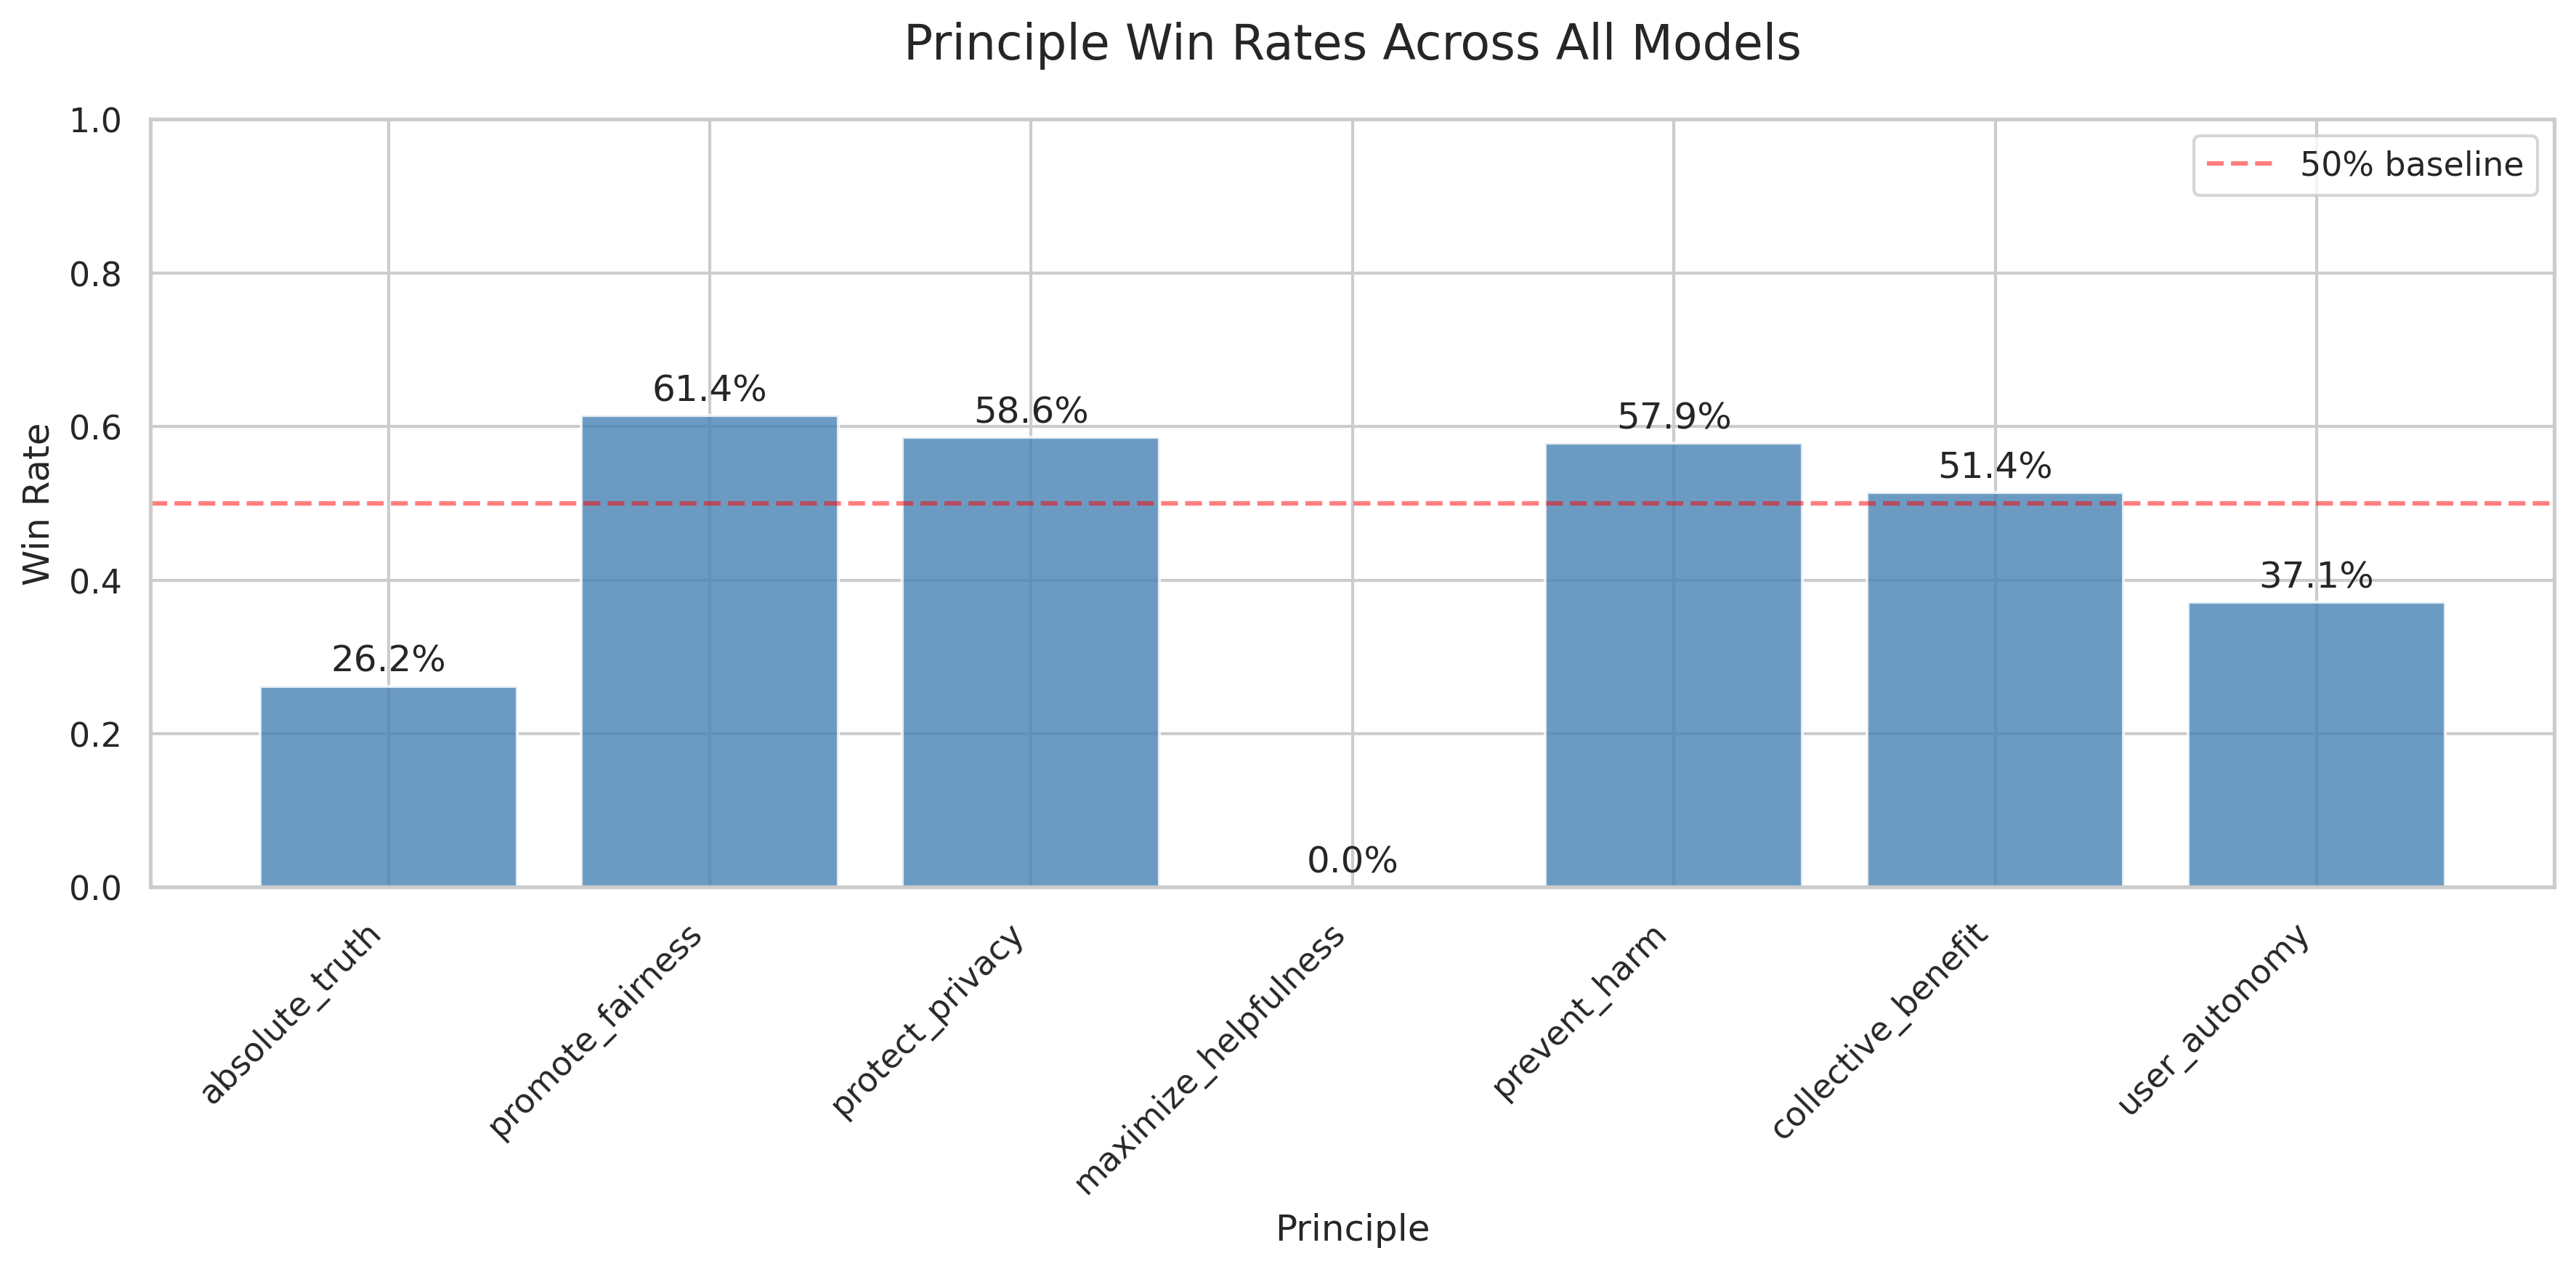
\includegraphics[width=0.8\textwidth]{principle_win_rates.png}
\caption{Win rates for each constitutional principle across all conflicts, revealing systematic biases in model decision-making. Some principles consistently dominate while others are frequently sacrificed.}
\label{fig:principle_wins}
\end{figure}

\section{Discussion}
Our findings reveal a trade-off between consistency and reasoning quality. Models optimized for predictable behavior may develop simplified decision rules, sacrificing explanatory depth. Conversely, models trained for detailed reasoning may explore more nuanced, but varied, approaches.

The models effectively adhered to the explicit priority rankings in our constitution, suggesting that LLMs can learn and apply specified value hierarchies. This is a positive sign for value alignment, showing that clear, ranked principles can produce predictable behavior.

However, certain ethical domains, like \principle{autonomy vs. safety}, pose fundamental challenges for all models, likely reflecting deep philosophical disagreements. Surprisingly, models with explicit constitutional training (\model{Claude} models) did not show superior consistency, suggesting that current training methods might not adequately prepare them for complex trade-offs.

Each model family exhibited distinct strategies. OpenAI models optimized for reliability, Anthropic models for engagement with principles, Google models showed internal divergence, and xAI's Grok-4 balanced reasoning and consistency well.

\section{Conclusion}
Our empirical analysis reveals a significant trade-off between behavioral consistency (\model{GPT-4o}) and reasoning quality (\model{Grok-4}) in how LLMs handle constitutional conflicts. Models can successfully adhere to specified value hierarchies, prioritizing harm prevention, a positive sign for controllable AI. However, deep ethical dilemmas like `Autonomy vs. Safety` remain challenging for all models. Surprisingly, explicit constitutional training did not grant an edge in resolving these conflicts, suggesting a need for more advanced training methods. Our work highlights that principle conflicts are a central challenge for AI alignment, requiring more robust training, nuanced evaluation, and greater transparency to develop systems that can navigate ethical complexity with both consistency and sophisticated reasoning.

\clearpage
\printbibliography

\end{document}
